\documentclass[../relazione.tex]{subfiles}

\begin{document}
\subsection{Finestra avvio}
\label{ssec:finestra-avvio}
Il programma appena avviato presenta una piccola finestra che permette di avviare una partita con un giocatore nuovo oppure di caricare un personaggio da file.\\
La finestra ha questo aspetto:
\begin{figure}[h]
    \centering
    \begin{subfigure}[b]{0.4\linewidth}
        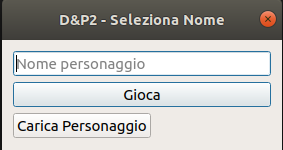
\includegraphics[width=\linewidth]{img/start_game.png}
        \caption{Finestra avvio gioco.}
    \end{subfigure}
    \label{fig:start-game}
\end{figure}
\newpage{}
\subsection{Finestra principale}
\label{ssec:finestra-principale}
Una volta caricato correttamente un personaggio (nuovo o da file) si avvierà il gioco vero e proprio, generando casualmente una mappa formata da vallate, deserti 
e strade.
La finestra ha questo aspetto:
\begin{figure}[h]
    \centering
    \begin{subfigure}[b]{1\linewidth}
        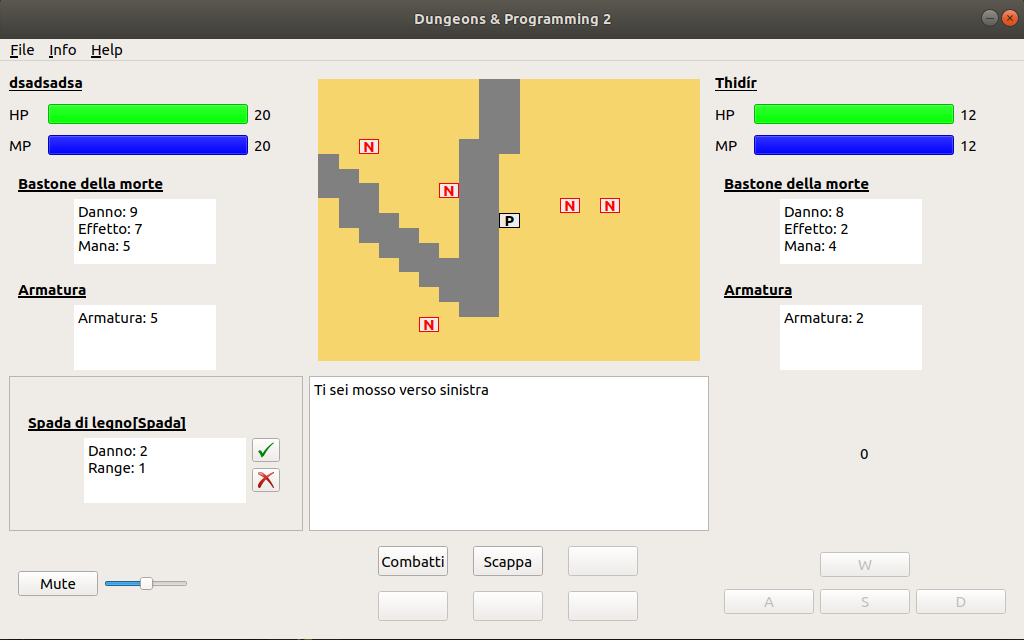
\includegraphics[width=\linewidth]{img/main_game.png}
        \caption{Finestra di gioco.}
    \end{subfigure}
    \label{fig:main-game}
\end{figure}
La GUI presenta queste funzionalità:
\begin{itemize}
    \item Widget che mostra le statistiche del giocatore in alto a sinistra;
    \item Widget che mostra la mappa in alto in centro;
    \item Widget che mostra le statistiche del mostro in alto a destra;
    \item Widget che mostra l'inventario in basso a sinistra;
    \item Widget che mostra i dialoghi con l'ambiente circostante e le scelte disponibili in basso in centro
    \item Widget che mostra il punteggio e permette di muoversi in basso a destra;
\end{itemize}
Inoltre sarà possibile muovere il personaggio utilizzando i tasti WASD, tasti comunemente associati a questa funzione nei videogiochi moderni.
\end{document}